\documentclass[12pt]{article}
\usepackage{amsmath,amssymb,amsthm}
\usepackage{fullpage}
\usepackage{graphicx}
\newtheorem{thm}{Theorem}[section]

\theoremstyle{definition}
\newtheorem{defn}{Definition}[section]
\newcommand{\floor}[1]{\left\lfloor #1 \right\rfloor}
\newcommand{\ceil}[1]{\left\lceil #1 \right\rceil}
\begin{document}
\title{Finding a non-constructively defined set of 6-cliques in an
$n$-vertex graph requires $\Omega(n^3)$ NAND gates}

\author{Josh Burdick ({\tt josh.t.burdick@gmail.com})}
\maketitle

I am writing this up on the assumption that it's not new.
However, I'm hopeful that either it is new, or that it has useful bits,
or that someone can point me
to similar lower-bound attempts. (Or if it's wrong, that 
someone can point out the flaw in the argument).

It's basically a function-counting argument; such arguments have been known for
a long time \cite{shannon_synthesis_1949}.

\tableofcontents

\section{A counting bound}

The first argument is basically a function-counting argument.

\subsection{Background: lower bounds from function counting}

It's long been known that computing {\em some} function of a bit-string
requires exponentially large circuits \cite{shannon_synthesis_1949}.
If there are $m$ inputs to a circuit,
then there are $2^{2^m}$ possible functions from the $m$-input bitstring to
a one-bit output. Each of these functions, being different, must have a
different circuit.

If we assume the circuit is made of NAND gates, and has $g$ gates, then the
circuit could have at most $gm$ wires from inputs to gates, and ${g \choose 2}$
wires from gates to gates. We can view the possible circuits as a bitmask,
containing a 1 everywhere a gate is connected to an input (or another gate),
and 0 everywhere else.

\begin{thm}
\label{boundFromCounting}
Consider functions from $m$ bits to one bit of output.
This means that, with $g$ gates, we can represent at most
$2^{gm + {g \choose 2}}$ different boolean functions (with $m$ bits of input,
and one bit of output).
\end{thm}
\begin{proof}

The number of possible wires which are there, or not, is $gm + {g \choose 2}$,
which bounds how many possible circuits there are.
Some of these circuits compute the same function.
However, there can't be any more than this many circuits with this many wires.
\end{proof}

This means that if we have a large set of functions, and we know the size of
the set of functions, then we know that at least {\em one} of them requires
a large number of gates. (Knowing {\em which} function requires a lot, or many,
gates is still an issue).

Consider functions from $m$ bits to one bit of output.
Let $g$ be the number of gates, and $w$ be the number of wires.
Solving for the number of gates:

\begin{eqnarray*}
w & = & mg + {g \choose 2} \\
  & = & mg + g(g-1)/2 \\
  & = & mg + (g^2 - g) / 2 \\
  & = & 0.5g^2 + (m-0.5)g \\
0 & = & 0.5g^2 + (m-0.5)g - w \\
\end{eqnarray*}

We solve the quadratic formula (writing $b = m-0.5$ for simplicity), keeping
only the non-imaginary root.

\begin{eqnarray*}
g & = & -b \pm \sqrt{ b^2 + 2w} \\
  & = & {\sqrt {2w + b^2}} - b \\
\end{eqnarray*}

Thus, given a set of functions, we know that at least one of them requires
some number of gates.

\subsection*{Bounding the average number of gates}

We can also count the total number of functions from $m$ input bits to one
output bit, using up to $g$ NAND gates, as

\begin{eqnarray*}
\sum_{i=0}^{g-1} 2^{m+i} & = & 2^{m+g} - 2^m
\end{eqnarray*}

If we're counting circuits with up to $g$ gates, then some of the circuits
have fewer than $g$ gates. This somewhat complicates the book-keeping.
However, {\em most} of the
circuits have $g$ gates. (Indeed, well over half, since each additional
gate adds many potential wires). Because of this, I think that the
average case bound is just one fewer gates than the worst-case bound.


\subsection{Counting CLIQUE-like functions}

We now consider NAND gate circuits (with any fan-in) which find $k$-cliques in $n$-vertex
graphs.

We consider the set of ``buggy'' 6-clique finders. 
Maybe the circuit correctly
finds all the cliques. Or maybe it finds all of the cliques except $K_{1..6}$,
or it misses half the cliques, or finds none (and always outputs 0), or maybe
it only successfully finds $K_{1,3,4,5,7,8}$, or whatever. More formally,
we define a set of functions ({\em not} circuits)

\begin{defn}
\label{BUGGY-6-CLIQUE}
${\rm BUGGY-6-CLIQUE}(n)$ is the set of functions which recognize any set
of $K_6$s. That is, for each set $A$ of $K_6$s, ${\rm BUGGY-6-CLIQUE}(n)$
contains a function which is 1 if the input contains any $K_6 \in A$,
and 0 otherwise.
\end{defn}

This clearly includes HAS-6-CLIQUE (which finds all the cliques).

These functions are all distinct. If $f_1, f_2 \in {\rm BUGGY-6-CLIQUE}(n)$,
then there's some $K_6$ such that if $y$ is the graph with {\em only}
1's in that $K_6$ (and 0's elsewhere), $f_1(y) = 0$ and $f_2(y) = 1$.

Of course, many of these functions are quite similar (e.g. all but one of them
output a 1 when you feed in all 1's). However, they're all slightly different.

\begin{thm}
\label{buggyDistinct}
${\rm BUGGY-6-CLIQUE}(n)$ contains $2^{n \choose 6}$ distinct functions.
\end{thm}
\begin{proof}
That's how many subsets of the $K_6$s there are.
\end{proof}

Although $2^{n \choose 6}$ is a fairly large number,
it's still comfortably less than $2^{2^{n \choose 2}}$, the number of boolean
functions on the ${n \choose 2}$ input wires to the circuit (there's one input
per edge in the input graph).

\subsubsection{But {\em which} function requires many gates?}

So, there are $2^{n \choose 6}$ different functions. 
How many NAND gates do these take?
(We onsider NAND gate circuits (with any fan-in) which find $k$-cliques in $n$-vertex
graphs, as a circuit with $n \choose 2$ inputs)

Applying Theorem
\ref{boundFromCounting}, we know that at least one of the circuits requires
${\sqrt {2 {n \choose 6} + b^2}} - b = \Omega(n^3)$ 
NAND gates (where $b = {6 \choose 2} - 0.5$).

Why doesn't this bound CLIQUE?
Because we don't know that the circuit which actually,
correctly, finds all of the
$K_6$s, is one of these larger circuits. As far as what I've
shown thus far goes, it could be harder to find some weird subset of the $K_6$s...

Indeed, as far as what I've formally shown goes, the problem which needs
the most NAND gates could be finding a single $K_6$! That's easily ruled out
(because that only needs one NAND gate, plus the output gate.)

\section{Other things about the counting bound}

These are some other thoughts about the counting bound, which didn't
seem to get me anywhere.

\subsection{Which sets of cliques are hard to find?}

We can also consider various subsets of the cliques. For instance,
most of the functions in BUGGY-k-clique find exactly
$0.5 {n \choose k }$ cliques. This means that, on average, these
require $\Omega(n ^ (k/2)$ gates to compute.

However, the hardness of these functions depends somewhat
on exactly how the cliques they find are laid out.
For instance, here are two sets of 20 triangles (that is, ``$K_3$s''),
arranged in different ways:

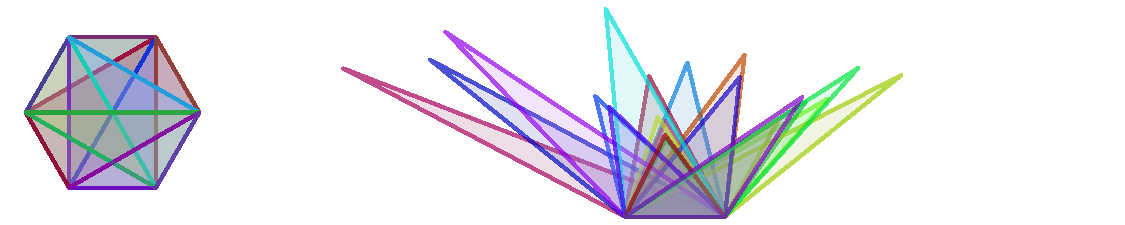
\includegraphics[width=0.9\textwidth]{R/tri1.pdf}

There are fast algorithms known for
detecting triangles using matrix multiplication
 \cite{itai_finding_1977} \cite{williams_multiplying_2012}, so
something like what's on the left can be done (for large enough
$n$) using fewer than ${n \choose 3}$ gates.

On the other hand, if the gates overlap less (as on the right),
then we will definitely need at least ${n \choose 3}$ NAND gates
(which is to say, more NAND gates).
To see this, note that if we feed in a 0 to the input for one
of the edges unique to some triangle, then any gate connected to
that edge will only output a 1. We can repeat this for each of the
triangles, constructing a series of strictly smaller circuits
(this is essentially what I think is called
the ``method of restrictions'' FIXME CITE).

Indeed, since we're using NAND gates, we know that finding any non-empty
subset of cliques is strictly harder than finding {\em some} other 
smaller set of cliques (namely, the set you get after feeding in 0's to
all the edges connected to some vertex).
Unfortunately, this doesn't help much
in the case of CLIQUE.  If we have a circuit which
finds $k$-cliques on 100 vertices, and feed in 0's to all edges connected to
one vertex, we
end up with... a strictly smaller circuit which finds $k$-cliques on
99 vertices! We still haven't connected the complexity of CLIQUE with
the complexity of all those ``buggy'' circuits which find exactly half
the cliques.


\subsection{Slightly larger sets of functions}

We can also construct somewhat larger sets of functions. For instance,
suppose that, rather than detecting or ignoring each clique, we assign
to each edge either 1, 0, or X, with this interpretation:

\begin{itemize}

\item 1: ``this clique must be present''

\item 0: ``this clique must NOT be present''

\item X: ``I'm ignoring this clique''

\end{itemize}

There are $3^{n \choose k}$ such strings. However, those consisting only of
0's and X's always output 0, and so are indistinguishable, so there are
only $3^{n \choose k} - 2^{n \choose k}$ distinct functions.

The lower bound on the average hardness of computing these functions is
slightly higher. However, this doesn't seem to help that much.

Note that distinguishing the functions requires that we be able to have at
least two distinct cliques either be present or absent. With two cliques,
we can do this by feeding in 1's to any edges shared by the cliques, and
then feed in 0's or 1's to the remaining edges:

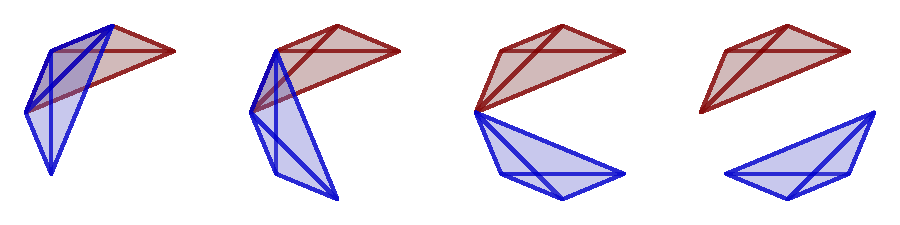
\includegraphics[width=0.7\textwidth]{R/overlapping.pdf}

However, it seems hard to push this to arbitrary functions of ``which cliques are
present'', because they start to overlap.

\section{Decomposing graphs into hypercliques}

Suppose we consider all $2^{n \choose k}$ functions which find some subset
of $k$-cliques in an $n$-vertex graph, and for each, find the circuit with
the fewest NAND gates which computes it. If we add up the total number of
gates in all of these circuits,
it's a lot. Since they're all distinct functions, the
function-counting bound should
allow us to lower-bound the total number of gates used (as from the
above, we know how many functions from $m$ inputs to one output
we can implement using $g$ NAND gates).

Note that, for a given set of $k$-cliques $S$, if $S = A \cup B$, and we
have circuits to find the $k$-cliques in $A$ and $B$, then by ORing them
together, we obtain a circuit for $S$. (With NAND gates, you actually
save a gate. Given circuits for $A$ and $B$, to construct a circuit
for $A \cup B$, you just disconnect the wires from $B$'s last gate, and
connect them to $A$'s last gate. $A$'s output now computes $A \cup B$,
and $B$'s last gate is no longer needed).

Suppose we had small circuits for detecting all of the $k$-cliques
in an $m$-vertex graph, for $k \le m \le n$.
Then, one way to generate a circuit which finds an arbitrary subset
of $k$-cliques would be to decompose it into a set of
cliques (of size between $k$ and $n$), and OR them all together.

Suppose we do this, for {\em all} of the $2^{n \choose k}$ possible subsets of
$k$-cliques. We then add up the total number of clique detectors of each
size that we've used, and total up how many NAND gates are in each of these.
We had better have used at least as many NAND gates as the Shannon counting
bound says we needed, to implement all of those functions.

Broadly speaking, the idea of using an upper bound to prove a lower bound
is not new. Aaronson describes this as ``ironic complexity theory''
\cite{aaronson_pnp}, and mentions several recent applications of it.

\subsubsection{Anecdotal rephrasing}

(I include the following hypothetical anecdotal explanation,
partly because I think it's slightly funny, but also because I think it may
provide at least some intuition).

In some alternate reality, it is the dawn of the era of 
TTL integrated circuits.
Yoyodyne Corporation has developed a line of integrated circuits to detect
any possible set of $K_4$s in a graph with nine vertices.
These chips, the 74LSC series,
are available in a convenient 40-pin DIP package, and are
fabulously successful. (I have no idea why there would be huge demand for
these, but let's say that there is). The only problem is that Yoyodyne's 
chip factories are having trouble producing enough chips.

Management contemplates how to re-envision productivity and enable
synergy. (They are, after all, producing $2^{9 \choose 4} = 2^{126}$
different sorts of chips).
They decide that they need to stop producing so many kinds of chips.
After great deliberation, they decide to cut production to {\em just} the
chips which find all possible
$K_4$'s on graphs with between four and nine vertices (namely, the 74LSC4
through 74LSC9). In order to meet the bizarre but humongous
demand for finding arbitrary sets of $K_4$s, they will develop a
line of tiny circuit boards,
each containing several clique detectors, ORed together.

There is still the problem of designing these circuit boards. However,
they only have to do this once for each possible set of $K_4$s. They hire
a large team of software engineers and graph theorists. By renting
many years of CPU time from AltaVista and MySpace, they are able to design the
optimal circuit boards.

Note that, originally, Yoyodyne was using some number of NAND gates to
cover all the $2^{9 \choose 4} = 2^{126}$ possible sets of $K_4$s.
The Shannon counting
argument gives a lower bound on how many NAND gates were used in all of
these chips. (Specifically, it says that at least four NAND gates
were used for at least one graph, since $36+37+38+39 = 150 \ge 126$).

After the redesign, if 
we count up the number of 74LSC4 through 74LSC9 gates which were used,
and consider the number of NAND gates in each
of these, the total had better {\em also} be larger than the bound from
the Shannon counting argument.

\subsubsection{Getting a bound from covering all the hypercliques}

Suppose we devise a way of covering all the $k$-cliques in an $n$-vertex
graph. Let

$A_{ij}$ = the average number of $i$-vertex cliques in a $j$-vertex graph

$b_i$ = the Shannon bound on the number of
gates needed to find $k$-cliques on $n$ vertices.

$x_j$ = the number of gates needed to find $k$-cliques on $j$ vertices.

If we have a covering strategy, and $A$ is the number of each size of
clique needed, then by the above argument, we have a bound $Ax >= b$.
This would give a lower bound on $x$ (the number of gates needed to find
$k$-cliques in $j$-vertex graphs.

(Note that I'm not necessarily saying the bound on $x$ is even positive...)

\subsection{How do we cover the graphs?}

Thus, we are faced with the problem of covering all possible $2^{n \choose k}$
sets of cliques with a small number of large cliques.
We can think of a set of possible $k$-cliques as
a $k$-regular hypergraph on $n$ vertices. The {\em density}
of such a graph is defined the fraction of possible edges which it contains,
$|E| / {n \choose k}$ \cite{keevash2011hypergraph}.
(I will often omit the ``hyper'' from
``hypergraph'', ``hyperedge'', etc.)

We have unlimited computational resources to cover the
graph with clique detectors of various sizes. However,
at the end of the day, we need to know (as precisely as possible)
how many clique detectors of each
size we're using (not just how many clique detectors were used).
For this to be efficient, we presumably need as many of
the cliques as possible to be large, and to not overlap much.

\subsubsection{Using the set-cover greedy algorithm}

Suppose we're given a $k$-regular (hyper)graph, and are trying to cover it
with a small number of (hyper)cliques. This is reminiscent of the
set cover problem, in which we are trying to cover some elements with
a small number of sets.
There is a greedy
strategy for set-cover, which consists
of simply picking the set which covers the most elements, removing those
elements, and repeating \cite{chvatal1979greedy}.
This has a guaranteed approximation ratio.

This suggests the following strategy. Pick the largest clique, remove it, and
repeat. If we do this, then each time we remove a clique, we know exactly
how much the density of the graph is reduced. If we known that a
sufficiently-dense graph has a fairly large clique, then we should be able
to bound how many cliques of each size we decomposed the original graph into.

It's known that if a conventional graph (that is, a graph
in which each edge has two vertices, or ``2-regular graph'')
has many edges, then it must contain
a clique of a certain size.
Finding the densest graphs which lack some size of clique was an
early problem in extremal graph theory. Since these maximally dense graphs
(the Tur\'an graphs) have a known structure, the size of the clique is
known precisely \cite{turan1941external}.

Generalizing this to hypergraphs seems like a natural question.
Based on the neatness of the solution for 2-regular graphs,
we might guess that, if we know that a $k$-regular hypergraph is dense,
then it must contain a fairly large clique, with a closed-form size.

Unfortunately, for hypergraphs, there doesn't seem to be as neat
an answer as there was for 2-regular graphs. 
There is a large gap in the density of graph having some size
of clique
\cite{keevash2011hypergraph}. That survey (p. 23-26)
describes the ``Tur\'an density'' $\pi(K^r_k)$,
which is $1 - t(k,r)$. The bounds on $t$ given there are

\[
{{k-1} \choose {r-1}}^{-1} \le t(k,r) \le \big(\frac{r-1}{ k-1 }\big)^{r-1}
\]

Given these bounds, in our running example of finding $K_6$s, at what density
of 6-regular graph are we guaranteed to find a $K^6_7$ -- that is, seven
vertices such that all possible edges of size 6 are included?
(The nomenclature here is different from what I've been using, which is
unfortunate.) It looks like, plugging in $k=7, r=6$, the bound doesn't
essentially
guarantee that there will be a $K^6_7$ until the density is
$1 - {6 \choose 5}^{-1} = 5/6$. Larger hypercliques will require even
higher densities.

If we choose a $k$-regular hypergraph uniformly at random,
``most'' of the subsets of cliques have density near 0.5. But at that density,
the known
bounds can't guarantee that there will be many cliques for us to cover.
Thus, it seems unlikely that
we can use this strategy to (non-constructively) cover the graph with
cliques. However, it is funny to consider that if we {\em could} find a
bound for $k$-regular graphs with $k \ge 3$
(for which Erd\"os offered \$1,000 \cite{keevash2011hypergraph}),
{\em and} it turned
out that the bound implied that sufficiently dense hypergraphs always had
``large'' hypercliques, then we also {\em might} have a
lower bound on CLIQUE.

\subsubsection{Using ``brute force'' to count large cliques / coverings}

It seems like, for {\em small} graphs, some of these questions could be
addressed (although not answered)
 using brute force. Suppose $n, k$ are small enough that we can 
store the adjacency matrix of a $k$-regular graph as a bitvector, and precompute
all possible hypercliques
(with up to $n$ vertices) as bitvectors. Then we can easily generate
random graphs (as bitvectors), count the cliques, and compare that to the graph
density. (Or possibly use the greedy set-cover strategy, and see how
many cliques are need, for random graphs).

I implemented this, and found that there was usually at least one small
hyperclique, basically in line with the predictions in \cite{bollobas1976cliques}
(data not shown).

\section{Non-constructively covering random hypergraphs}

The lack of large hypergraph Tur\'an bounds was initially discouraging.
However, that problem (which possibly founded extremal graph theory?) is
``extreme'' in the sense that it looks for the densest graph which lacks
a clique. It pays little attention to the average case.

Also, Keevah's review notes that when a hypergraph is dense enough to
definitely contain some subgraph, it's apt to contain that subgraph
``all over the place'' \cite{keevash2011hypergraph}, a phenomenon
known as ``supersaturation''.  This seems similar to what's
described in \cite{bollobas1976cliques}, which suggests that most of
the cliques in a random graph have a somewhat narrow range of sizes.
This suggests that even if there isn't definitely a huge hyperclique,
there may at least be many smallish hypercliques.
Indeed, \cite{bollobas1993clique} discusses covering graphs (not hypergraphs)
with many cliques of the same size.

Thus, we try to use random graph theory to upper-bound how many
$r$-vertex clique detecters (on average, or total). We will actually
try to use all of the maximal cliques in a graph (that is, all of the
cliques which are not part of a larger clique). This is presumably
somewhat inefficient.
For instance, in this toy example in which we're covering edges
(``$K_2$''s), there
are three maximal $K_3$s, but we could get by with two $K_3$s and
a $K_2$. Presumably similar things happen with hypergraphs.

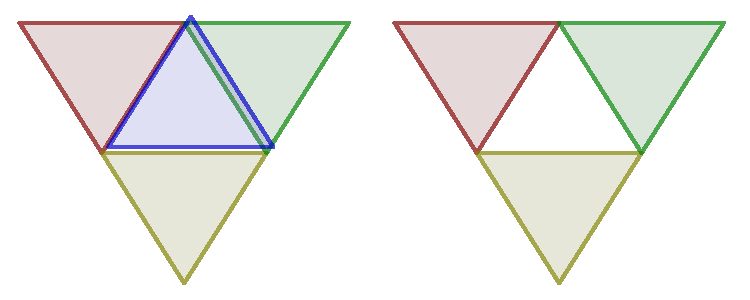
\includegraphics[width=0.7\textwidth]{R/maximal.pdf}


\subsubsection{How many hypercliques in a random hypergraph?}

One model of random graphs
includes each edge with some fixed probability. Using this model,
\cite{bollobas1976cliques}
counts the expected number of hypercliques in a hypergraph. Assuming all
edges are chosen i.i.d. (in our case, with probability 1/2),
there are ${n \choose r}$ possible $r$-vertex hypergraphs which might
occur. Each of these is present if ${r \choose k}$ edges are present; as it
were, if that many coins all come up heads. Then the total number of times
we expect this to happen, as noted in \cite{bollobas1976cliques}, is

\[
{n \choose r} \cdot 2^{-{r \choose k}}
\]

Note that these could very well overlap. However, this isn't a problem for
us in terms of correctness. If we cover some clique
with more than one
clique detector, we're
ORing all the detectors together anyway. (This may be wasteful, and it's
possible that we could manage better by only using some of the inputs to
some clique detectors. For now, we ignore this possibility.)

\subsubsection{How often do big hypercliques cover smaller ones?}

The above bound counts hypercliques of different sizes, but has much overlap.
Every time the graph contains a 15-vertex hyperclique, that includes
15 14-vertex hypercliques, ${15 \choose 13}$ 13-vertex hypercliques,
tons of 8-vertex hypercliques, etc. We want to
cover this with one 15-vertex clique detector.

Instead, we consider the odds of a given $r$-vertex hyperclique $A$
being completely
covered by an $r+1$-vertex hyperclique. This requires, for a given vertex
$v$, that all ${r \choose {k-1}}$ edges (consisting of $v$ plus $k-1$ vertices
of $A$) be present. $v$ could be any of $n - r$ vertices; if at least one
 of those
``completes'' $A$, then $A$ is covered. We're interested in counting the
probability that this {\em doesn't} happen (as that's the number of smaller
hypercliques we need to cover). That fraction is

\[
\Big[1 - 2^{-{r \choose {k-1}}}\Big]^{n - r}
\]

In concrete terms, if we consider when $k=6$, suppose that hyperedge
1..6 is present.
The odds of a given vertex ``extending'' that hyperedge to a 7-vertex
hyperclique are $2^{-{6 \choose 5}} = 2^{-6} = 0.015625$, since all
64 other hyperedges need to be present. If the total number of vertices $n=7$,
then there's about a 98\% chance of {\em not} extending
this to a larger hyperclique. However, as $n$ gets large, there's more chance
of a larger hyperclique
happening. When $n=1000$, most hyperedges will be part of a larger
hyperclique. Even if you're batting .015, in 1,000 at-bats, you're apt to
get a hit...

However, when we consider larger $r$-vertex hypercliques, with $r > k$,
the odds of the hyperclique being covered by a larger hyperclique decrease
really fast. Then again, when $r = n/2$, there are lots of hypercliques...

Thus, it's not obvious (to me)
how these two opposing trends will play out. However, these
expressions do at least seem to give a bound on the total number of
hypercliques needed.

\subsection{A bound based on covering hypergraphs with cliques}

To conclude this section, here is a bound based on covering hypergraphs
with hypercliques.
If we know the average number of gates needed to find many sets of cliques, and
can do that efficiently using a ``small'' number of clique detectors,
then we hopefully get a bound on the number of gates in each clique detector.

On the left side, we have
the Shannon bound on how many gates are needed, for an average function
chosen randomly from BUGGY-$k$-CLIQUE.

On the right side, we have
the average number of gates which suffice for us to cover the hyperedges
(which are $K_k$s in the original input graph) of an instance of
BUGGY-$k$-CLIQUE.
We will assume that we can detect $k$-cliques on $r$-vertex graphs using
$h(r)$ NAND gates, for some function $h$.
We then sum up the total cost (in NAND gates)
of covering that many $r$-vertex hypergraphs in a larger $n$-vertex graph.

\[
\underbrace{\sqrt{n \choose k} - {n \choose 2}}_\text{average number of gates needed}
\le \sum_{r=k}^n
\underbrace{h(r)}_\text{cost, in gates}
\cdot
\underbrace{{n \choose r} \cdot 2^{-{r \choose k}}}_\text{expected number of $K_r^k$s}
\cdot
\underbrace{\Big[1 - 2^{-{r \choose {k-1}}}\Big]^{n - r}}_\text{fraction of $K_r^k$s not covered by a $K_{r+1}^k$}
\]

We then hope that if we set $h$ to, say, a small enough
function, we'll get a contradiction.

I tried to simplify this formula (e.g. by trying to change it into an
integral), without much luck.
However, even
without simplifying this formula more, we could imagine computing $A$ and
$b$ for a range of $n$ and $k$, and solving for the minimum values of
$x$ (a lower bound on the
number of gates needed) using a linear program solver.
I haven't done this so far.

\subsection{Using just one size of hyperclique}

As that expression is complicated, we seek a simpler (but
presumably slacker) bound.

As noted earlier, there is a strong incentive to use the largest
hypercliques possible, as our assumption is that this will be less
expensive. However, we don't expect large hypercliques to be frequent.
Still, 
\cite{bollobas1993clique} covers random graphs with cliques of just
one size.

This suggests the simpler strategy of picking one intermediate
size of hyperclique,
and only use clique-finding for that size problems. For smaller problems,
just use one NAND gate per hyperedge (clique).
This presumably is less efficient, but might be easier to analyze.

Furthermore, I only belatedly realized that the above bound is about
finding $k$-cliques in $r$-vertex graphs; $n$ can be chosen to optimize the
bound.

In terms of the previous metaphor, perhaps Yoyodyne has abandoned trying to
create a custom chip for every possible hypergraph. Instead, they have
developed a CISC chip
with a CLQ instruction, which checks for a clique
of any given size. But then, a contingent of chip architects, fresh from
reading \cite{hennessy2011computer}, argue that they're better off building
a chip with a CLQ instruction which only works for a fixed size of graph.
Maybe this simplifies pipelining the clique detector...

\subsubsection{Measuring the cost}

Suppose that we pick $r$ such that $k < r < n$; in the given hypergraph,
we will cover every $K_r^k$ with some circuit; all remaining hyperedges
(cliques) will simply be detected with one NAND gate each.

The left-hand side is the Shannon bound on the average number
of gates.

Assume that this subcircuit, for finding $k$-cliques in an $r$-vertex graph,
requires $h(r)$ NAND gates, for some
function $h$. Then,
the cost to cover all edges in a $K_r^k$ is simply $h(r)$ times the
expected number of $K_r^k$s (as estimated in \cite{bollobas1976cliques}).
This is the first term below.

How many edges are left over? These are ``expensive'', as we're
paying one gate for each. How likely is an edge to be ``missed''
by the larger cliques? There are $k$ edges in the clique, so to form
the larger clique, we need to pick $r-k$ additional vertices from
the $n-k$ vertices not in the edge. Given that edge is chosen, there
are another ${r \choose k} - 1$ edges which all have to be included,
each with probability $1/2$.
This is the second term below.

\[
\underbrace{\sqrt{n \choose k} - {n \choose 2}}_\text{Shannon bound}
\ge
\underbrace{\frac{1}{2} {n \choose r} (1 - 2^{1-{r \choose k}}) ^ {n-k \choose r-k}}
_\text{Gates for edges not covered by a clique}
   + \underbrace{h(r) \cdot {n \choose r} 2^{-{r \choose k}}}
_\text{Gates for edges covered by a clique}
\]

The nice thing about this sum is that it's only two terms (rather than
the summation above).

\subsubsection{Checking the amount of coverage}

These predictions made me slightly wary, as the events they were counting
aren't independent.
We can numerically check the predicted number of cliques
of various sizes from \cite{bollobas1976cliques}.
(In the following graphs, the dotted line is the prediction, and
the solid line is the average of samples).

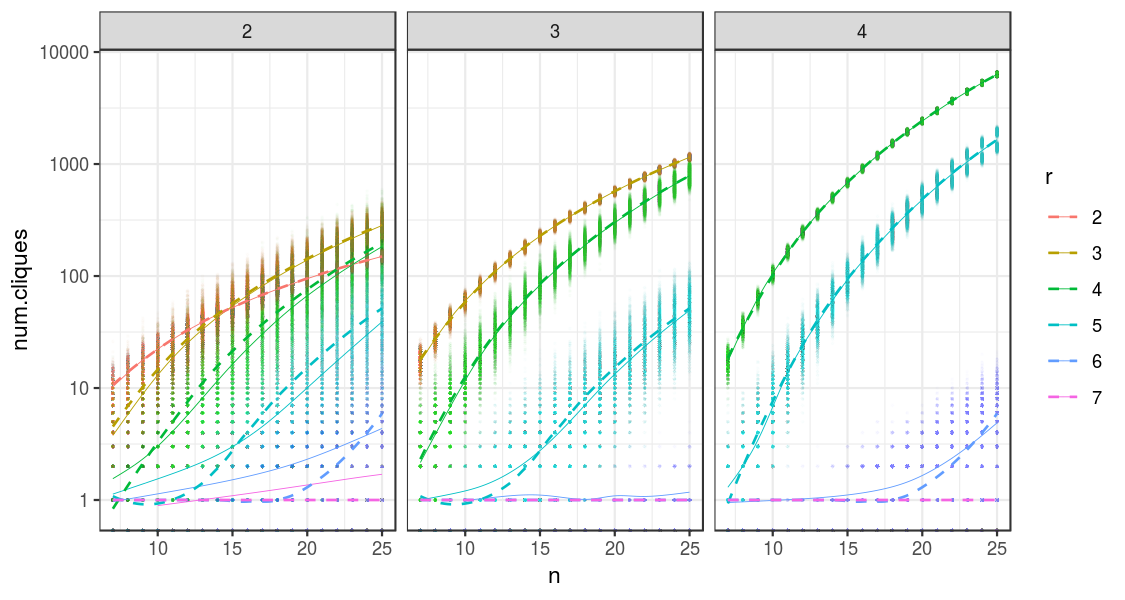
\includegraphics[width=1\textwidth]{cliqueCounter/R/numCliques.png}

We can also count the number of edges covered for different sizes
of edge:

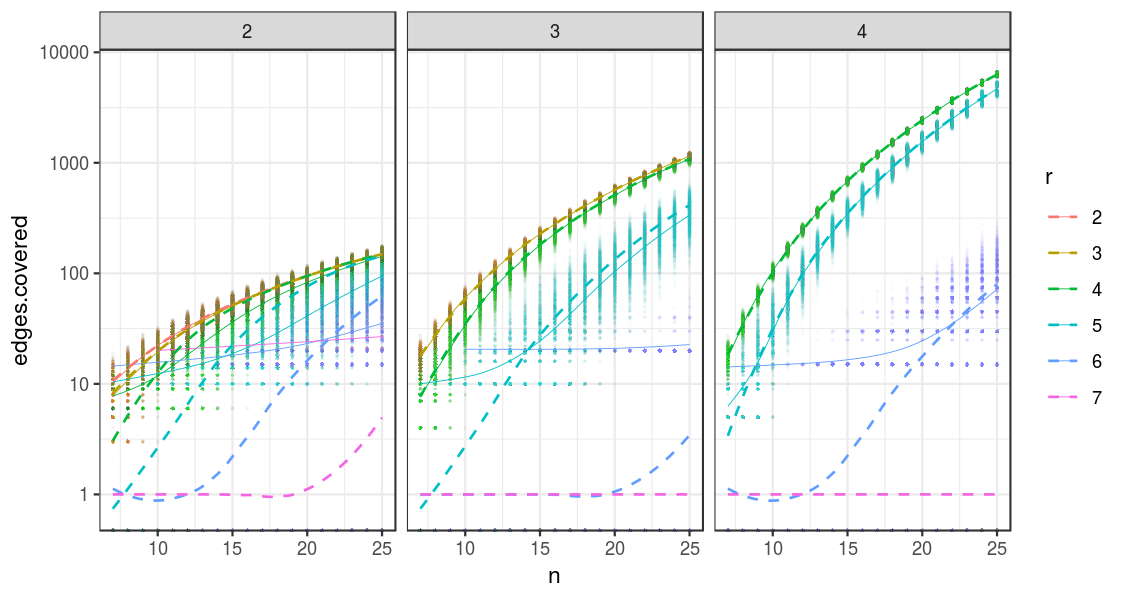
\includegraphics[width=1\textwidth]{cliqueCounter/R/edgesCovered.png}

More relevant to this problem, is the fraction of edges covered
by one of the r-cliques:

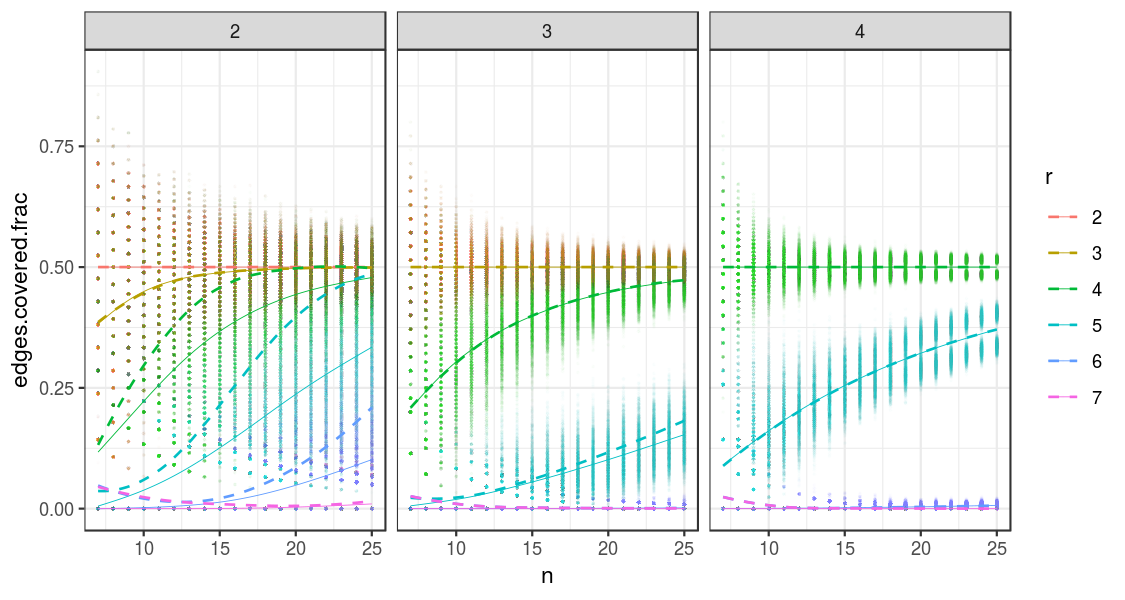
\includegraphics[width=1\textwidth]{cliqueCounter/R/fracCovered.png}

All of these
estimates appear more accurate for larger edge sizes and graphs, which
makes sense to me, because of the Central Limit Theorem.

I then attempted to maximize this for a tiny case, $k=5$ and $r=6$.
(Initially in R, and then using Julia's arbitrary-precision arithmetic,
in an attempt to deal with the large numbers). Searching for $n$ up to 500,
this did eventually get above zero.
The maximum was when $n=420$, at which point the bound was
... $3.1355 \cdot 10^{-6}$.

Since there must be an integral number of NAND gates, we can then round up
to ``at least one NAND gate.''
(This is reminiscent of the ``chipmunks in trees''
problem (\cite{ross2006first}, p. 344). However, this doesn't help much.

\section{Conclusion}

We first give a lower bound on finding {\em some} set of cliques.
It is a modified form of Shannon's counting argument
\cite{shannon_synthesis_1949}.

We also present a connection between this argument and the problem of covering
hypergraphs with hypercliques.
It seems that if an arbitrary hypergraph can be covered with 
``large'' hypercliques,
then this would give a lower bound on the NAND gates required to
detect cliques.

However, using one (relatively simple) strategy for doing this covering,
the bound was, like, less than one. Possibly improving the covering
strategy would help, but I'm not convinced it would help much.

(If it's the case that any function in BQP can be represented
as a circuit made of discrete quantum gates, which can be
ORed together, then this also
would imply that BQP doesn't contain NP).

\bibliography{references}
\bibliographystyle{abbrv}

\end{document}

